\documentclass[10pt]{IEEEtran}
\usepackage{import}

\usepackage{amssymb}
\usepackage{amsmath}
\usepackage{amsthm}
\usepackage{mathtools}
\usepackage{thmtools}
\usepackage[margin=.75in]{geometry}
\usepackage{enumerate}
\usepackage{tasks}
\usepackage{graphicx}
\usepackage{xcolor}
\usepackage{bm}
\usepackage{fancyhdr}
\setlength{\headheight}{15pt}
\usepackage[T1]{fontenc}
\usepackage{float}
\usepackage{ifthen}
%\usepackage{bbold}
\usepackage{multicol}
\usepackage{blkarray}
\usepackage[framemethod=TikZ]{mdframed} %For MD Theorem

\usepackage{cancel}
\usepackage[mathscr]{euscript}

\newlength{\drop}

%%%%% Tuyen Macros
\theoremstyle{plain}
\newtheorem{theorem}{Theorem}
\newtheorem*{theorem*}{Theorem}%[section]
\newtheorem{example}{Example}%[section]
\newtheorem{defi}{Definition}%[section]
\newtheorem{cor}{Corollary}%[section]
\newtheorem{lemma}[theorem]{Lemma}
\newtheorem{proposition}{Proposition}
\newtheorem*{proposition*}{Proposition}

\renewcommand{\iff}{\Leftrightarrow}
\renewcommand{\phi}{\varphi}
\renewcommand{\epsilon}{\varepsilon}
\renewcommand{\indent}{\hspace{\parindent}}
\newcommand{\ceil}[1]{\lceil #1\rceil}
\newcommand{\floor}[1]{\lfloor #1\rfloor}
\newcommand{\intd}{\,\text{d}}
\newcommand{\normal}{\trianglelefteq}
\newcommand{\tor}{\operatorname{Tor}}
\newcommand{\st}{\,:\,}
\newcommand{\divides}{\bigm|}
\newcommand{\cl}[1]{\overline{#1}}
\newcommand{\syl}{\text{Syl}}
\newcommand{\gen}[1]{\left\langle{#1}\right\rangle}
\newcommand{\sclabel}[1]{\underset{#1}{\operatorname{\_}}}
\newcommand{\remmelArrow}[1]{\operatornamewithlimits{\longrightarrow}^{(#1)}}
\newcommand{\Z}{\mathbb{Z}}
\newcommand{\N}{\mathbb{N}}
\newcommand{\R}{\mathbb{R}}
\newcommand{\Q}{\mathbb{Q}}
\newcommand{\C}{\mathbb{C}}
\newcommand{\F}{\mathbb{F}}
\newcommand{\bd}{\partial}
\newcommand{\card}{\operatorname{card}}
\newcommand{\ckr}{\text{coker}}
\newcommand{\im}{\text{im}}
\newcommand{\aut}{\operatorname{Aut}}
\newcommand{\gal}[1]{\operatorname{Gal}(#1)}
\newcommand{\quot}[2]{\left.\raisebox{.2em}{$#1$}\middle/\raisebox{-.2em}{$#2$}\right.}

\newcommand{\secSplit}{
\begin{center}
    \makebox[2in]{\hrulefill}
\end{center}}

%%%%%%%%% Community Macros (You can parse this out per person if you want)

\newcommand{\ra}{\rightarrow}
\newcommand{\lr}{\leftrightarrow}
\newcommand{\0}{\varnothing}
\renewcommand{\Z}{\mathbb{Z}^+}
\renewcommand{\R}{\mathbb{R}}
\renewcommand{\C}{\mathbb{C}}
\newcommand{\An}{A_n}
\newcommand{\U}{\bigcup_{n=1}^{\infty}}
\newcommand{\Uj}{\bigcup_{j=1}^{\infty}}
\newcommand{\UN}{\bigcup_{n=N}^{\infty}}
\newcommand{\UUN}{\bigcap_{n=N}^{\infty}}
\newcommand{\Ua}{\bigcup_{\An\subset A}}
\newcommand{\UU}{\bigcap_{n=1}^{\infty}}
\newcommand{\A}{\mathscr{A}}
\newcommand{\M}{\mathscr{M}}
\newcommand{\g}{\gamma}
\newcommand{\s}{\sigma}
\newcommand{\la}{\lambda}
\renewcommand{\S}{\sum}
\renewcommand{\d}{\delta}
\newcommand{\m}{\mu}


\newtheorem*{problem}{Problem}
\newtheorem*{solution}{Solution}
\usepackage{tikz}
\usepackage{tikz-cd}


\usetikzlibrary{shapes.geometric}
\newcommand{\contradiction}{
\begin{tikzpicture}[x=0.5ex,y=0.5ex]
\draw (-.25,-.25)--(2,2) (0,2)--(2.25,-0.25) (-.25,.75)--(1,-.5)--(2.25,.75);
\end{tikzpicture}}

\usetikzlibrary{decorations.pathreplacing,angles,quotes}
\usetikzlibrary{decorations.markings}

\tikzset{edge/.style = {shorten >=0.5em,shorten <=.5em, ->}}
\tikzset{marr/.style = {decoration={markings, mark=at position 0.625 with {\arrow{>}}}, postaction={decorate}}}
\tikzset{rmarr/.style = {decoration={markings, mark=at position 0.375 with {\arrow{<}}}, postaction={decorate}}}
\tikzset{mmarr/.style = {decoration={markings, mark=at position 0.6 with {\arrow{> >}}}, postaction={decorate}}}
\tikzset{none/.style = {}}

\newcommand{\lattice}[2]{
	\foreach \x in {0,1,...,#1}{
		\foreach \y in {0,1,...,#2}{
			\node[draw,circle,inner sep=1.5pt,fill] at (\x,\y) {};
		}
	}
}
\newcommand{\Look}{\hspace{-.75em}
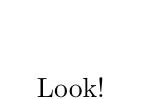
\begin{tikzpicture}[baseline=-.8ex]
\node[] at (0,0) {Look!};
\path [draw] (-.18,-.2) to [out=-60, in=-120] (.11,-.2);
\end{tikzpicture}}

\newcommand{\axes}[4]{
    \draw[<->, thin] (#1,0)--(#3,0);
    \draw[<->, thin] (0,#2)--(0,#4);
    \draw[thin, dotted] (#1,#2) grid (#3, #4);
}
\newcommand{\commutes}[3]{
    \draw[-latex, domain=180:490, variable = \x] plot ({#1+(#3)*cos(\x)},{#2+(#3)*sin(\x)});
}



\title{Gait Lab Project}
\author{
    \IEEEauthorblockN{John Hanlon} \IEEEauthorblockA{UF College of Veterinary Medicine} \\
    \and \IEEEauthorblockN{Andrew Jensen} \IEEEauthorblockA{UF College of Engineering}
}




\begin{document}
\maketitle
    \section{Introduction}
    The human musculoskeletal system's primary function is to support our bodies' dynamic and loaded motion. In order to better understand the underlying pathologies of the musculoskeletal system, researchers have sought to understand the joints' motion. One such way to measure the kinematics of the joints is using motion capture, which takes advantage of an over-constrained system of externally-placed markers tracked by a series of high-speed cameras. This report outlines how to measure the knee's kinematics during various activities dynamically. These results will then be compared with proprietary gait lab software to determine how well our manual calculations line up.

    \section{Methods}
    \subsection{Experimental}
    A young, healthy, male test subject was selected for use in this joint kinematic assessment. Marker placement related to the assessment of right knee kinematics were present on the right medial and lateral femoral epicondyles, the anterior aspect of the right thigh mid-way between the right knee and right hip joints and the anterior aspect of the proximal right tibia (maximal point of tubial tuberosity). The marker placed on the right medial femoral epicondyle was removed following assessment of the markers in a static pose prior to initiation of dynamic evaluation. Additional markers were placed but data collected from their positioning was not used for this project but could be used for calculation of additional reference frames for evaluation of kinematics of other joints. \\
    Motion capture was performed with the subject on a treadmill set to a walking and running speed of 2.8 mph and 5.0 mph respectively. An incline was then placed on the treadmill to simulate uphill running at a speed of 5.2 mph and additional  motion capture data was collected. 
    \subsection{Computational}
    First, we want to define a reference frame for the femur. We do this during the static pose (or T-pose) trial. These matrices will be saved for later use.
\begin{equation}
    \begin{aligned}
        \hat{O}_{fem} &= \frac{RMedKnee + RKnee}{2}\\
        \hat{x}_{fem} & = \frac{RKnee - RMedKnee}{\|RKnee - RMedKnee\|} \\
        \hat{z'}_{fem} &= \frac{HJC - O_{fem}}{\|HJC - O_{fem}\|} \\
        \hat{y}_{fem} &= \frac{\hat{z'}_{fem} \times \hat{x}_{fem}}{\|\hat{z'}_{fem} \times \hat{x}_{fem}\|} \\
        \hat{z}_{fem} & = \frac{\hat{x}_{fem} \times \hat{y}_{fem}}{\|\hat{x}_{fem} \times \hat{y}_{fem}\|}
    \end{aligned}
    \label{fem_rf}
\end{equation}
    
    Now, with an origin an three orthonormal basis vectors, we can create a reference frame,
    \begin{equation}
        \begin{aligned}
            T^{G}_{fem} &= \begin{bmatrix}
                \hat{x}_{fem} &\hat{y}_{fem} &\hat{z}_{fem} & O_{fem} \\
                0 & 0 & 0 & 1
            \end{bmatrix} \\
            &= \begin{bmatrix}
                & R^{fem}_{3 \times 3} & & O^{fem}_{3 \times 1} \\
                0 & 0 & 0 & 1
            \end{bmatrix}
        \end{aligned}
        \label{t_gf}
    \end{equation}

    Unfortunately, due to the removal of the $RMedKnee$ marker during dynamic activity, we aren't able to measure this reference frame dynamically. In order to do that, we need to create a fiducial reference frame that CAN be measured dynamically, then define the transform between this fiducial frame and the femur. We define this reference frame using the $RThigh$, $HJC$, and $RKnee$.
    Using a similar process as (\refeq{fem_rf}, \refeq{t_gf}), we obtain a similar transformation matrix $T^{G}_{thigh}$. 

    Now, we can define a reference frame $T^{thigh}_{fem}$, which we can use to post-multiply $T^{G}_{fem}$. 
    \begin{equation}
        T^{thigh}_{fem} = [T^{G}_{thigh}]^{-1}T^{G}_{fem}
    \end{equation}

    Now, for any dynamically measurable $T^{G}_{thigh}$, we can obtain the location of the femur via (\refeq{t_th_g_f}).

    \begin{equation}
        T^{G}_{fem,dynammic} = T^{G}_{thigh,dynamic}T^{thigh}_{fem}
        \label{t_th_g_f}
    \end{equation}

    \begin{mdframed}
        \subsubsection*{A Brief Example}
        Let's imagine we are trying to determine the location of the femur at $t=1.05s$, which occurs at the 655th frame. 
        
        First, we would use the process defined in (\refeq{fem_rf}, \refeq{t_gf}) to build a reference frame for the $RThigh$ at $t = 1.05s$. Then, with this reference frame defined for that particular time point, we can post-multiply by $T^{thigh}_{fem}$ in order to obtain $T^{G}_{fem}$.
        \begin{equation}
            T^{G}_{fem,dynamic} = T^{G}_{thigh,dynamic}T^{thigh}_{fem}
        \end{equation}
    \end{mdframed}

    Now, the ultimate goal is measuring the relative motion between the tibia and femur. To do this, we need to create some reference frames for the tibia. Similar to the femur, our desired reference frame (tibia) is not measurable dynamically due to the lack of markers. Thus, we create a similar fiducial markerset for the shank in order to measure the dynamic motion of the tibia.

    \begin{equation}
        \begin{aligned}
            \hat{O}_{tib} &= \frac{RMedKnee + RKnee}{2}\\
            \hat{x}_{tib} & = \frac{RKnee - RMedKnee}{\|RKnee - RMedKnee\|} \\
            \hat{z'}_{tib} &= \frac{RAnkle - O_{tib}}{\|RAnkle - O_{tib}\|} \\
            \hat{y}_{tib} &= \frac{\hat{z'}_{tib} \times \hat{x}_{tib}}{\|\hat{z'}_{tib} \times \hat{x}_{tib}\|} \\
            \hat{z}_{tib} & = \frac{\hat{x}_{tib} \times \hat{y}_{tib}}{\|\hat{x}_{tib} \times \hat{y}_{tib}\|}
        \end{aligned}
        \label{tib_rf}
    \end{equation}

    \begin{equation}
        \begin{aligned}
            T^{G}_{tib} &= \begin{bmatrix}
                \hat{x}_{tib} &\hat{y}_{tib} &\hat{z}_{tib} & O_{tib} \\
                0 & 0 & 0 & 1
            \end{bmatrix} \\
            &= \begin{bmatrix}
                & R^{tib}_{3 \times 3} & & O^{tib}_{3 \times 1} \\
                0 & 0 & 0 & 1
            \end{bmatrix}
        \end{aligned}
        \label{t_gt}
    \end{equation}
    Much like above, this can only be measured statically, so we must create a fiducial marker set that can be measured dynamically, and relate the two with a transformation matrix. We do this using the three points $RShank$, $RAnkle$, and $RKnee$, using a similar process outlined above.

    \subsubsection{Relative Tibiofemoral Motion}
    At this point, we are able to dynamically determine the location of our femur and tibia in the global reference frame. Using the multiplicative and invertible properties of the transformation matrices, we can determine the relative transformation between the femur and tibia (\ref{t_fem_tib}).

    \begin{equation}
        \begin{aligned}
            T^{fem}_{tib} &= [T^{G}_{fem}]^{-1}T^{G}_{tib} \\
            &= [T^{G}_{thigh}T^{thigh}_{fem}]^{-1}[T^{G}_{shank}T^{shank}_{tib}]
        \end{aligned}
        \label{t_fem_tib}
    \end{equation}
    This matrix gives us the relative position and rotation between our femoral and tibial reference frames. Decomposing this matrix into the multiplication of X-Y-Z rotations, we can extract the anatomic rotations as flexion/extension, varus/valgus, and internal/external (\refeq{rot}).

    \begin{equation}
        \begin{aligned}
            R^{fem}_{tib} & = R_{x}R_{y}R_{z}\\
            &= \begin{bmatrix}1 & 0 & 0 \\ 0 & c_{x} & -s_{x} \\ 0 & s_{x} & c_{x} \end{bmatrix}
            \begin{bmatrix}c_{y} & 0 & s_{y}\\ 0 & 1 & 0 \\ -s_{y} & 0 & c_{y} \end{bmatrix}
            \begin{bmatrix} c_{z} & -s_{z} & 0 \\ s_{z} & c_{z} & 0 \\ 0 & 0 & 1 \end{bmatrix}\\
            &= \begin{bmatrix}
                c_{y}c_{z} & -s_{z}c_{y} & s_{y} \\
                s_{z}c_{x} + s_{y}s_{x}c_{z} & -s_{x}s_{y}s_{z} + c_{x}c_{z} & -c_{y}s_{x} \\
                -c_{z}c_{x}s_{y} + s_{x}s_{z} & s_{z}s_{y}c_{x} + c_{z}s_{x}  & c_{x}c_{y}
            \end{bmatrix}
        \end{aligned}
        \label{rot}
    \end{equation}

    We can decompose this into our desired angles using basic trigonometry.

    \begin{equation}
        \begin{aligned}
            \theta_{x} & = tan^{-1}(-\frac{R_{2,3}}{R_{3,3}}) = \text{Flexion/Extension}\\
            \theta_{y} &= sin^{-1}(R_{1,3}) = \text{Abduction/Adduction} \\
            \theta_{z} & = tan^{-1}(-\frac{R_{1,2}}{R_{1,1}}) = \text{Internal/External Rotation} \\
        \end{aligned}
    \end{equation}

    \section{Data Assessment}
    \subsection{Repeatability of Knee Angles Within the Same Test Conditions}
    \subsubsection{Walking}
    The previously described protocol for joint angle calculation produced consistent and repeatable joint angles in flexion, adduction/abduction and internal/external rotation during both the swing and stance phase of the gait cycle when compared between strides. Though small variation between cycles is present, this variance is likely due to true variance in joint angle caused by minor variation in the gait between steps taken (stride length, relative step placement, etc.). 
    \subsubsection{Running}
    The previously described protocol generated consistent joint angles when compared between strides in flexion, abduction/adduction and internal/external rotation. Again, though minor variation was present between gait cycles, this variation is likely due to changes in the characteristics of the gait as no two strides will be exactly identical in all aspects. 

    \subsection{Comparison of Joint Angles}
    \subsubsection{Comparison of Walking and Running Knee Joint Angles}
    Knee joint angles measured during running are consistently greater in all axis in comparison to those measured during a walk. Maximal knee flexion, though present during the swing phase in both conditions, was 32\% greater during running, increasing from 74.4 degrees to 98.2 degrees from walking to running respectively and correspond to a larger stride length and necessity to generate increased force during the running condition. A proportionally greater increase in stance phase maximal knee flexion angle was appreciated during running, attributable to the greater vertical force experienced by the knee during the stance phase of the gait cycle during running compared to walking. A large increase in knee abduction/adduction joint angle was appreciated when running that, though possibly representative of true tibial varus/valgus, may also be a misrepresentation of the true angle caused by combinations of other concurrent knee movements such as knee flexion and internal/external rotation as well as concurrent internal/external rotation of the hip, resulting in a false reading of the joint angle in the frontal plane. 
    \subsubsection{Comparison of Running on Flat Ground vs Running on an Incline}
    Large variation was only observed in knee flexion angles when compared between test conditions with flat ground running creating a maximal knee flexion angle of 98.2 degrees while 120.7 degrees of maximal flexion was appreciated during running on an incline. This supports what is expected considering the conditions as increased hip and knee flexion during the swing phase of the gait cycle is required during inclined conditions to account for the elevation increase if the same stride length is to be maintained. 

    \subsection{Comparison of Knee Flexion Angles with Lab Standard Software}
    \emph{Disclaimers:}
    \begin{enumerate}
        \item The provided data from the lab standard software is in the form of graphs which does not provide exact values for knee flexion at different points in e gait cycle. Instead, only approximations of joint angles at different points in the gait cycle can be made. 
        \item Provided data from the lab standard software only includes knee flexion angles, not permitting comparison of other knee angles such as abduction/adduction or internal/external rotation. 
        \item The lab standard software data for knee flexion angles is reported as an average between all gait cycles included in the study period. This comes in comparison to the calculated maximal flexion values for a subset of gait cycles analyzed. True comparison would require mean maximal knee flexion angle for the calculated data or comparison of maximal flexion angles measured for the exact same gait cycle, which is not available from the lab standard software as provided. 
    \end{enumerate}

    \subsubsection{Walking}
    During the walk, the maximal flexion angle calculated was 74.4 degrees, observed during mid to late swing phase of the gait cycle. Though the maximal flexion angle was measured during the same point in the gait cycle by the lab standard software, the maximal flexion angle measured by the software was approximately 20 degrees less at around 55 degrees. (see disclaimers A and C for potential contributions to this discrepancy).
    \subsubsection{Running}
    Similar to the comparison between software for walking, knee joint flexion angle and adduction/abduction measures were calculated as greater using the described methods compared to the standard lab software. The maximal flexion angle calculated was 98.2 degrees while the maximal flexion calculated by the lab standard software was roughly 90 degrees. This discrepancy is very similar to the differences in calculated values for the walking condition. (see disclaimers A and C for potential contributions to this discrepancy).
    \subsubsection{Inclined Running}
    An increased difference was appreciated when comparing knee flexion angle between lab standard values and calculated values during inclined running conditions. Calculated maximal flexion angle was 120.7 degrees compared to an average of approximately 90 degrees from the lab standard software. (see disclaimers A and C for potential contributions to this discrepancy).

\end{document}